\chapter{A partilha do relógio}\label{cap:partilha}

O capítulo da intervenção terminou com uma dívida declarada: se o orçamento é um só, os dias gastos
segurando o mundo para conhecê-lo são dias em que o sistema não aprende nada de novo. A pergunta
que sobra é a da travessia entre proteger e adaptar: \textbf{recalibrar a barreira compete com acompanhar
o mundo?}

\section{A barreira tem dois ingredientes}

A barreira desta travessia é o produto de duas coisas, e as duas não se comportam do mesmo jeito\cite{sebastian2025enhancing}.

\begin{definicao}[escala e forma]\label{def:escala-forma}
A \emph{escala} de um dia é o nível da oscilação, estimado com os dias anteriores a ele. A
\emph{forma} é o corte da série já dividida pela escala: quantas vezes o nível a barreira fica acima
dele. A barreira do dia é o produto da escala pela forma.
\end{definicao}

A escala é a média de \numPartilhaJanelaEscala{} dias, e a forma é o \numPartilhaPosto{}º maior dos
últimos \numPartilhaJanelaForma{} dias padronizados. Os dois números são escolhas declaradas. O que se
mede não depende deles.

A moeda também precisa ser dita antes de ser usada, e é a natural de quem protege: a soma do que
passou por cima da barreira, dia a dia. Uma moeda só, para os dois ingredientes, de modo que comparar
não exige declarar um câmbio entre coisas diferentes.

O defeito que este capítulo mede é o palpite simétrico: tratar proteger e acompanhar como dois
consumidores iguais do mesmo relógio, e repartir o orçamento de atualizações meio a meio.

\section{As duas pressas}

O mundo da medição é uma série de \numPartilhaDiasDeSerie{} dias que dobra a sua oscilação de uma
vez, a um quarto do caminho. A avaliação olha os \numPartilhaHorizonte{} dias seguintes à mudança, em
\numPartilhaSementes{} mundos sorteados, e a dispersão vem junto.

O controle é o mesmo desenho num mundo que não muda: ali a perda absorvida é de
\numPartilhaPisoParado{} por dia, com dispersão de \numPartilhaPisoParadoDispersao{}. É contra esse
piso que as demais contas se leem.

\begin{figure}[htbp]
  \centering
  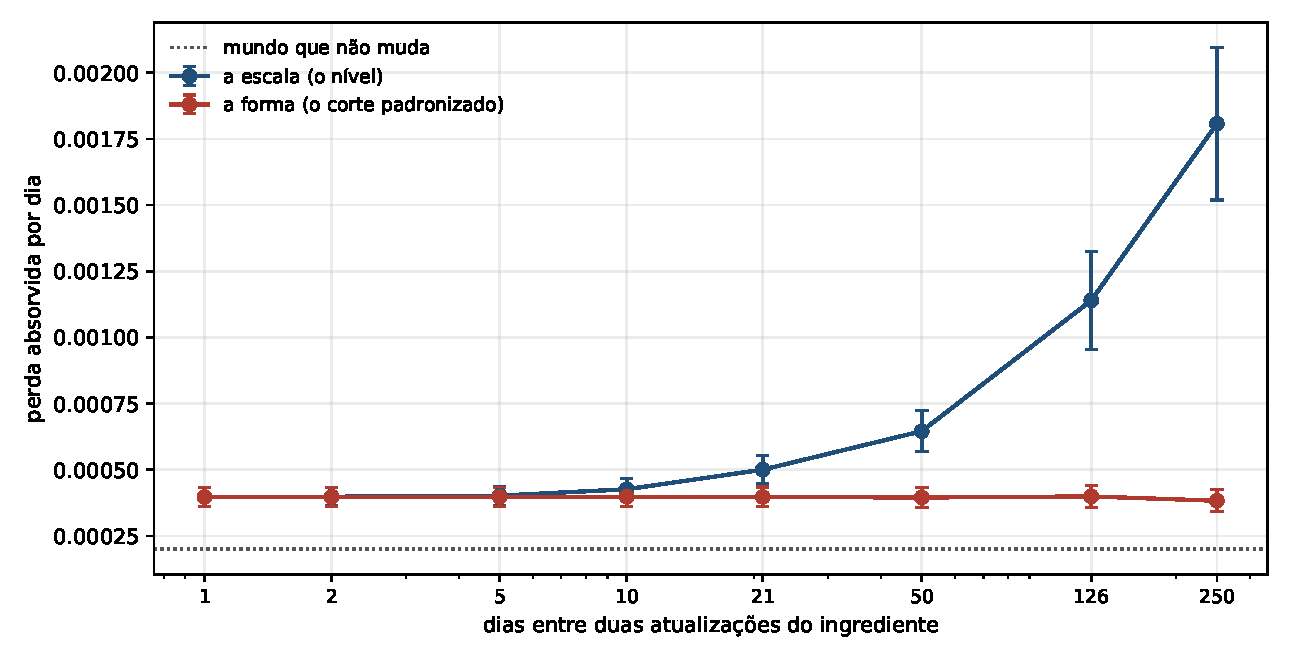
\includegraphics[width=\linewidth]{figuras/E11_partilha_do_relogio_1.pdf}
  \caption{A perda absorvida contra o tempo entre duas atualizações, atualizando um ingrediente por
    vez. O eixo dos tempos é logarítmico, de modo que a distância entre as últimas marcas vale muito
    mais dias do que a figura sugere. A linha pontilhada é o mesmo desenho num mundo que não muda.}
  \label{fig:duas_pressas}
\end{figure}

Atualizar a escala todo dia custa \numPartilhaEscalaDia{} de perda por dia; deixá-la envelhecer
duzentos e cinquenta dias custa \numPartilhaEscalaLenta{}, \numPartilhaRazaoEscala{} vezes o valor de
todo dia. A forma, medida do mesmo jeito, sai de \numPartilhaFormaDia{} para \numPartilhaFormaLenta{} ---
uma razão de \numPartilhaRazaoForma{}. As duas pressas diferem por quase cinco vezes de um lado e
por nada do outro.

A razão disso não é um acidente da medição, e vale escrever a conta que a sustenta.

% aterramento: padronizacao
% aterramento: c
\textbf{Padronizar} é dividir cada dia pela escala daquele dia: o valor padronizado é o afastamento
do dia medido em unidades do tamanho típico de então, e é ele que diz se o dia foi grande ou pequeno
para o mundo daquele momento. A letra $c$ é a constante positiva que multiplica a série inteira até
um instante, e a proposição diz o que acontece com a série padronizada quando o mundo todo cresce de
tamanho.

\begin{proposicao}[a escala some na padronização]\label{prop:padronizacao}
Se a série for multiplicada por uma constante positiva $c$ até o instante $t$, a série padronizada
não muda em nenhum instante até $t$. Em particular o corte da forma é o mesmo, e só a escala
carrega a mudança.
\end{proposicao}

\begin{proof}
A escala estimada em $t$ é a média dos dias anteriores a $t$; multiplicando a série por $c$, essa
média fica multiplicada por $c$. O valor padronizado é a razão entre o dia e a sua escala, de modo
que o $c$ do numerador e o $c$ do denominador se cancelam. O corte é um posto dessa razão, e um
posto não muda quando todos os seus valores são multiplicados pela mesma constante.
\end{proof}

Uma mudança que só multiplica a oscilação é invisível para a forma e é tudo para a escala. Por isso
a forma pode ser atualizada de vez em quando e a escala precisa ser atualizada sempre: cada uma
carrega a parte da mudança que a outra não vê\cite{borkar1997stochastic}.

\section{A partilha}

Com um orçamento de \numPartilhaOrcamento{} atualizações ao longo dos \numPartilhaHorizonte{} dias
de avaliação, a divisão pode ser medida inteira.

\begin{table}[htbp]
  \centering
  \small
  \begin{tabular}{rrr}
    \hline
    fração do orçamento & perda absorvida & \\
    que vai para a escala & por dia & \\
    \hline
    nenhuma & \numPartilhaSemAtualizarEscala & a escala fica velha \\
    metade & \numPartilhaMeioAMeio & o palpite simétrico \\
    \numPartilhaMelhorFracao & \numPartilhaMelhor & o melhor desenho medido \\
    \hline
  \end{tabular}
  \caption{A partilha do orçamento de \numPartilhaOrcamento{} atualizações. O desvio entre os \numPartilhaSementes{} mundos sorteados está na \cref{fig:partilha}. A
    fração que falta em cada linha vai para a forma.}
  \label{tab:partilha}
\end{table}

Deixar a escala sem atualização nenhuma leva a perda a \numPartilhaSemAtualizarEscala{},
\numPartilhaRazaoSemEscalaSobreMelhor{} vezes o valor do melhor desenho. Repartir meio a meio dá
\numPartilhaMeioAMeio{}, e a melhor partilha
medida é a de \numPartilhaMelhorFracao{} do orçamento para a escala, com
\numPartilhaMelhor{} --- \numPartilhaGanhoMeioAMeioPct\% menos perda do que o palpite simétrico, com
o mesmo trabalho.

O melhor ponto medido fica antes do extremo, e a diferença entre ele e dar tudo à escala é pequena ---
pequena o bastante para não se ler sem a dispersão. A partilha certa não é a igualitária nem a extrema\cite{grossberg1987competitive}.

\section{Quando a partilha morde}

Falta o controle que separa o que é do desenho do que é da pobreza do orçamento. Apertando o
orçamento e repetindo a mesma pergunta:

\begin{table}[htbp]
  \centering
  \small
  \begin{tabular}{rrr}
    \hline
    atualizações & perda com quase & ganho sobre o \\
    no horizonte & toda a escala & meio a meio \\
    \hline
    cinco & \numPartilhaQuaseTodaCinco & \numPartilhaGanhoCincoPct\% \\
    vinte & \numPartilhaQuaseTodaVinte & \numPartilhaGanhoVintePct\% \\
    sessenta & \numPartilhaQuaseTodaSessenta & \numPartilhaGanhoSessentaPct\% \\
    duzentos e cinquenta & \numPartilhaQuaseTodaDuzentosECinquenta & \numPartilhaGanhoDuzentosECinquentaPct\% \\
    \hline
  \end{tabular}
  \caption{O ganho de partilhar bem, contra o tamanho do orçamento. Com orçamento folgado, dividir de
    qualquer maneira dá quase o mesmo.}
  \label{tab:aperto}
\end{table}

Com cinco atualizações no horizonte, a partilha de \numPartilhaMelhorFracao{} do orçamento para a escala vale
\numPartilhaGanhoCincoPct\% menos perda do que o palpite simétrico;
perda; com duzentos e cinquenta, vale \numPartilhaGanhoDuzentosECinquentaPct\%. A competição que a
pergunta supõe existe, e aparece no aperto: enquanto houver atualizações de sobra, os dois
ingredientes recebem o que precisam e não disputam nada.

A última conta fecha o sentido do capítulo. Manter os dois ingredientes atualizados todo dia, ao
longo de \numPartilhaSobraAtualizacoes{} dias, leva a perda a \numPartilhaSobra{}, com desvio de
\numPartilhaSobraDispersao{} entre os mundos sorteados. O melhor desenho com \numPartilhaOrcamento{}
atualizações no mesmo horizonte fica em \numPartilhaMelhor{}: \numPartilhaApertoSobreTudoPct\% de
perda a mais, na média. A diferença é pequena e não se repete em todo mundo. Comparados par a par
nos mesmos \numPartilhaSementes{} mundos sorteados, o orçamento apertado entrega mais perda em
\numPartilhaApertoMundosQuePerdemContagem{} deles e menos nos
\numPartilhaApertoMundosQueGanhamContagem{} restantes, porque a diferença entre os dois desenhos
mede \numPartilhaApertoPorMundo{} de perda por dia e o desvio dessa diferença entre os mundos é
\numPartilhaApertoPorMundoDispersao{}, maior que ela. A pergunta que fica não é se vale a pena,
mas quanto se está disposto a pagar por um punhado de perda.

\begin{figure}[htbp]
  \centering
  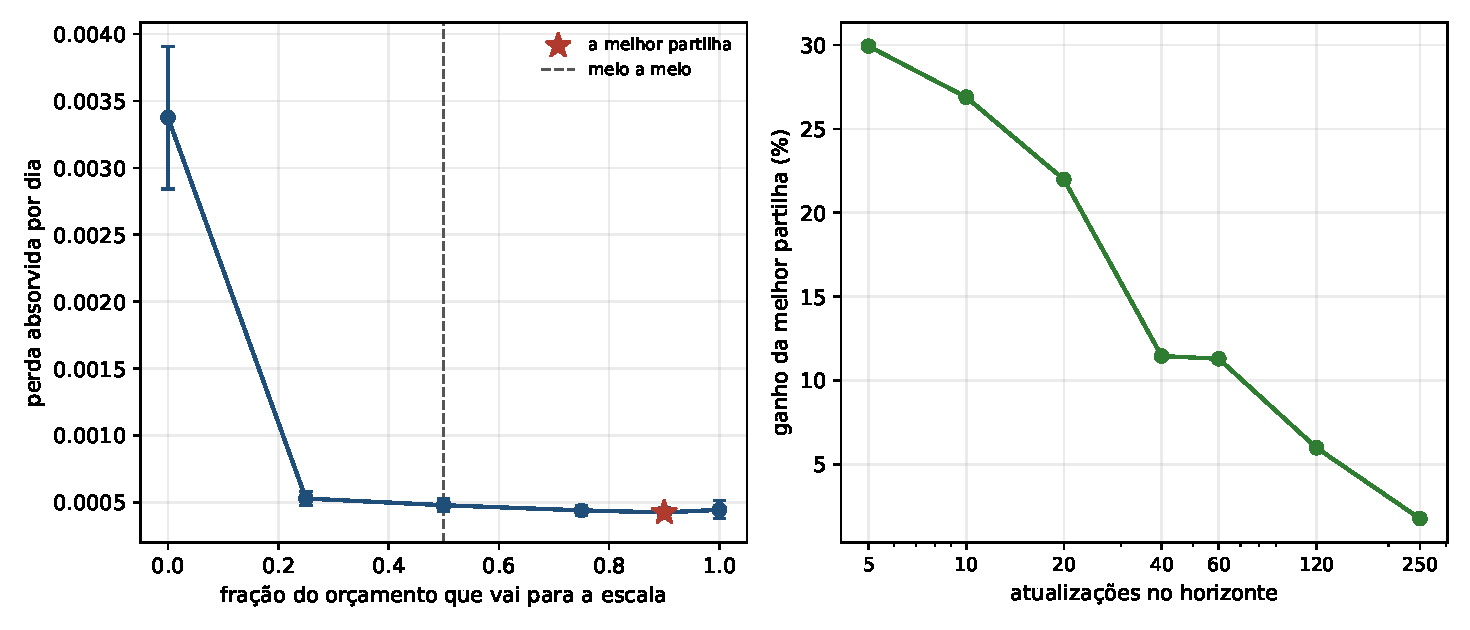
\includegraphics[width=\linewidth]{figuras/E11_partilha_do_relogio_2.pdf}
  \caption{À esquerda, a perda contra a fração do orçamento que vai para a escala, com a dispersão
    entre mundos. O eixo da fração é linear, de modo que os três últimos pontos ficam amontoados à
    direita. À direita, o ganho da melhor
    partilha de \numPartilhaMelhorFracao{} do orçamento para a escala contra o tamanho do orçamento: a
    vantagem de escolher bem encolhe quando o orçamento
    engorda.}
  \label{fig:partilha}
\end{figure}

\section{O que fica}

Fica a resposta da travessia, e ela separa duas coisas que a pergunta juntava. Os dois ingredientes
da barreira não competem pelo dado: o dado é o mesmo fluxo, não se gasta, e cada um pode ter a sua
janela sem tirar nada do outro. O que se gasta é o \textbf{trabalho} de refazer a conta, e aí a
competição é real --- com um desequilíbrio que a proposição explica: a escala carrega tudo o que a
mudança mexeu e a forma não carrega nada, de modo que quase todo o orçamento vai para um lado.

E fica o limite honesto do achado. A competição só morde quando o orçamento é pobre; com
atualizações de sobra, os dois recebem o que precisam e o desenho da partilha deixa de importar.
Isso também é resposta: o refutador declarado da pergunta era um orçamento em que os dois de fato
não competem, e ele existe --- é o orçamento folgado.

O fracasso seguinte está no próprio desequilíbrio que a partilha mediu. A escala é a que precisa ser
atualizada sempre, e atualizar é, no fundo, \textbf{esquecer}: cada atualização troca passado por
presente, e quanto mais depressa a escala acompanha, menos passado ela carrega. Quanto do passado se
pode apagar antes que o sistema deixe de aprender, ninguém mediu ainda, e é essa a próxima conta.
